\section{Elastic Sigmoid Curve}

We evaluate the Elastic Sigmoid Curve (ESC) as follows:

\begin{equation} \label{esc}
    c(r,t) = c_0 + \frac{(K-c_0)t}{r+t}
\end{equation}

where $t$ designates the time, $c_0$ is the initial condition and lower boundary at $t=0$, $K$ is the upper boundary with $\lim_{t \to \infty} c(r,t) = K$, and $r$ is a variable depending on the senders and receivers governance token holdings and how much liquidity they provide. It defines the gradient of the curve. The reward value $c(r,t)$ is added as a multiplier coefficient to the TRF introduced in the previous section. In the future we will add more reward multipliers based on governance decisions, e.g. for the type of transaction and where the transaction occurs.

(7) is modeled after the the law of diminishing returns, with a range from $c_0 \leq c(r,t) \leq K,\: \forall t > 0$. It is designed to keep up utility and liquidity for fluid derivatives and to incentivise users to hold their governance tokens in custody. A normalized graph of (\ref{esc}) can be seen below in \autoref{fig2}.

\begin{figure}[hb]
    \centering
    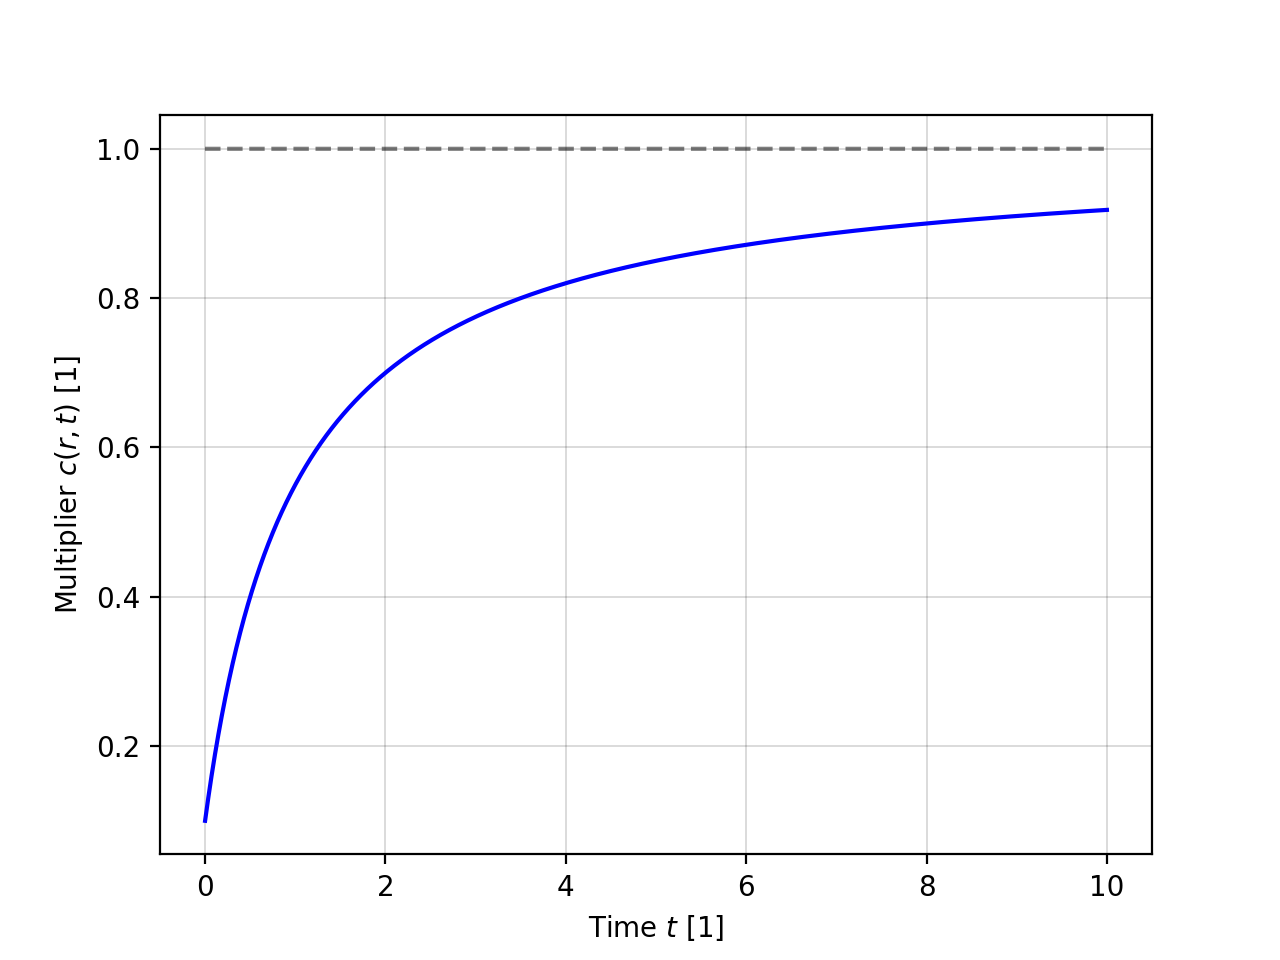
\includegraphics[width=10.5cm]{images/ESCnew.png}
    \caption{Normalized isoline of the ESC, $r=1,\: c_0 = 0.1,\: K=1$} \label{fig2}
\end{figure}

Users will be able to trade and lend their individual rewards on marketplaces ("Outcome Farming"). Once they remove liquidity or unlock their governance tokens, $c(r,t)$ will be reset accordingly based on the percentage of the withdrawn or sold assets. Further design considerations and how to evaluate the reward value $r$ will be discussed in a follow up paper. 

In the next section we introduce Fluidity's drawing mechanism for the dividend system to obtain the probability vector $p_m$.